% Source: https://tex.stackexchange.com/a/726764/6880

\documentclass[margin=2pt]{standalone}
\usepackage{tikz}
\usetikzlibrary{backgrounds}

\definecolor{myblue}{HTML}{2E7CAA}
\definecolor{mybluegray}{HTML}{5A7890}
\definecolor{myred}{HTML}{E72B22}
\definecolor{mydarkred}{HTML}{DE5744}
\definecolor{mycyan}{HTML}{BDE2ED}
\definecolor{mydarkcyan}{HTML}{2DA5BC}
\definecolor{mypurple}{HTML}{C29DE5}
\definecolor{mybrown}{HTML}{935134}
\definecolor{mylightgray}{HTML}{D1D6D9}

\begin{document}
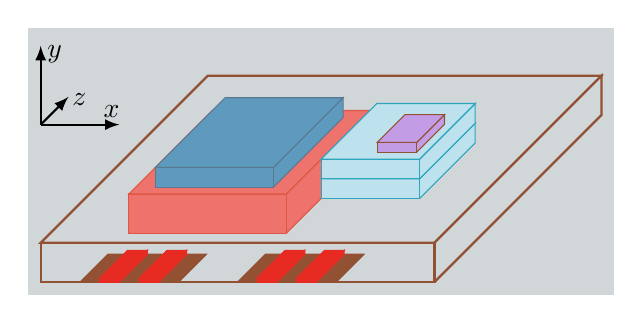
\begin{tikzpicture}[
z={({0.5cm*cos(45)},{0.5cm*sin(45)})},
% Cuboid ===============
pics/cuboid/.style n args={5}{
code={%%
\coordinate(A1) at (0,0);
\coordinate(B1) at (#1,0);
\coordinate(C1) at (#1,#2);
\coordinate(D1) at (0,#2);
\coordinate(B2) at (#1,0,#3);
\coordinate(C2) at (#1,#2,#3);
\coordinate(D2) at (0,#2,#3);
\path[draw=#4, fill=#5] (B1) -- (B2) -- (C2) -- (C1);
\path[draw=#4, fill=#5] (A1) rectangle (C1); 
\path[draw=#4, fill=#5] (D1) -- (C1) -- (C2) -- (D2) --cycle;
},%%
},% ==================
background rectangle/.style={draw=none, fill=mylightgray}, 
show background rectangle,
]

\draw (0.5,0,1.75) pic {cuboid={2}{0.5}{3}{mydarkred}{myred!66}};
\draw[] (0.75,0.5,2) pic {cuboid={1.5}{0.25}{2.5}{mybluegray}{myblue!77}};

\draw (2.5,0,3) pic {cuboid={1.25}{0.25}{2}{mydarkcyan}{mycyan}};
\draw (2.5,0.25,3) pic {cuboid={1.25}{0.25}{2}{mydarkcyan}{mycyan}};

\draw (3.125,0.5,3.25) pic {cuboid={0.5}{0.125}{1}{mybrown}{mypurple}};

\pic[thick]{cuboid={5}{0.5}{6}{mybrown}{none}};

\draw (0.5,0,0) pic {cuboid={1.25}{0}{1}{mybrown}{mybrown}};
\draw (0.75,0,0) pic {cuboid={0.25}{0.05}{1}{myred}{myred}};
\draw (1.25,0,0) pic {cuboid={0.25}{0.05}{1}{myred}{myred}};

\draw (2.5,0,0) pic {cuboid={1.25}{0}{1}{mybrown}{mybrown}};
\draw (2.75,0,0) pic {cuboid={0.25}{0.05}{1}{myred}{myred}};
\draw (3.25,0,0) pic {cuboid={0.25}{0.05}{1}{myred}{myred}};

%% CoSy
\begin{scope}[-latex, shift={(0,2)},thick]
\foreach \P/\s/\Pos in {(1,0,0)/x/above, (0,1,0)/y/right, (0,0,1)/z/right} 
\draw[] (0,0,0) -- \P node[\Pos, pos=0.9,inner sep=2pt]{$\s$};
\end{scope}
\end{tikzpicture}
\end{document}
